
\graphicspath{ {\curdir/Graphics/}  }

Surface electrode traps have several advantages over standard ``macro'' ion traps.  They can be repeatably manufactured and provide a large number of independent dc voltage parameters that can be used to precisely control the location and motion of trapped ions.  The difficulty in working with these traps is the decreased distance between the ions and the nearest surface.  Material deposited on these surfaces during the vacuum bake out or from the ovens can be charged and induce stray fields and additional heating on the ions.  Characterizing both of these problems is important for being able to perform high fidelity work in these systems.  We have performed some initial characterization of surface traps that we have been working with.  

\section{Ion Dark Lifetime}
\label{sec:lifetime}

One of the initial difficulties with working with surface traps was their poor ion lifetimes.  Even while being cooled ions would only stay trapped for minutes, and, without continuous cooling, lifetimes were often as small as a few seconds.  The first trap that we performed measurements in was a Sandia National Labs ``Y'' trap.  This surface electrode trap has three arms extending radially from a central point where they are all connected.  The radial trap is formed by rf and dc rails that run along the side of each arm.  Near the end of each arm there is a 100~micron by 100~micron hole through the entire chip that allows neutral atom flux to travel from behind the trap to be loaded into the trapping region above it.

Cooled lifetimes in this trap were easily tens of minutes, and further investigation of them would have been painfully slow so we performed measurements of the dark, uncooled lifetime instead.  An automated loading procedure was developed leveraging our TTL control over all ionization lasers and our neutral atom oven.  This system allowed the entire experiment to be automated even though it involved losing and retrapping ions many times.

Measuring dark lifetimes itself is straightforward.  A single ion is trapped and cooled using our normal cooling apparatus.  The cooling lasers are then well shuttered for a fixed period of time during which the ion is expected to heat.  The cooling lasers are then unshuttered and fluorescence is collected to determine if the ion remained in the trap.  If it did not, another ion is trapped, and then the experiment is repeated.

This measurement is expected to give some insight into the heating rate of ions in the trap.  The heating rate of ion traps is complicated but is related to the stray field and electric field noise environments of the ion.  Using our shuttling system we were able to repeat the measurement at different location along one arm of the trap.  It was expected that because of the neutral atom flux deposited underneath the loading hole this region could develop a large stray vertical electric field which would increase heating in this region.  

Motional heating in ion traps is a complicated phenomenon and is only recently beginning to be investigated systematically.  There are a number of phenomena known to cause heating including rf electric field noise near trap junctions, DAC sampling noise, and electric field noise at the secular frequencies \cite{Blakestad:09, Blakestad:11}.  The first heating source is significant in junctions in surface traps because there may be significant gradients in the rf pseudopotential.  The update rate of the DACs has strong frequency components that can cause direct heating of motional modes or combinations of motional modes through parametric resonances.

\begin{figure}
	\centering
	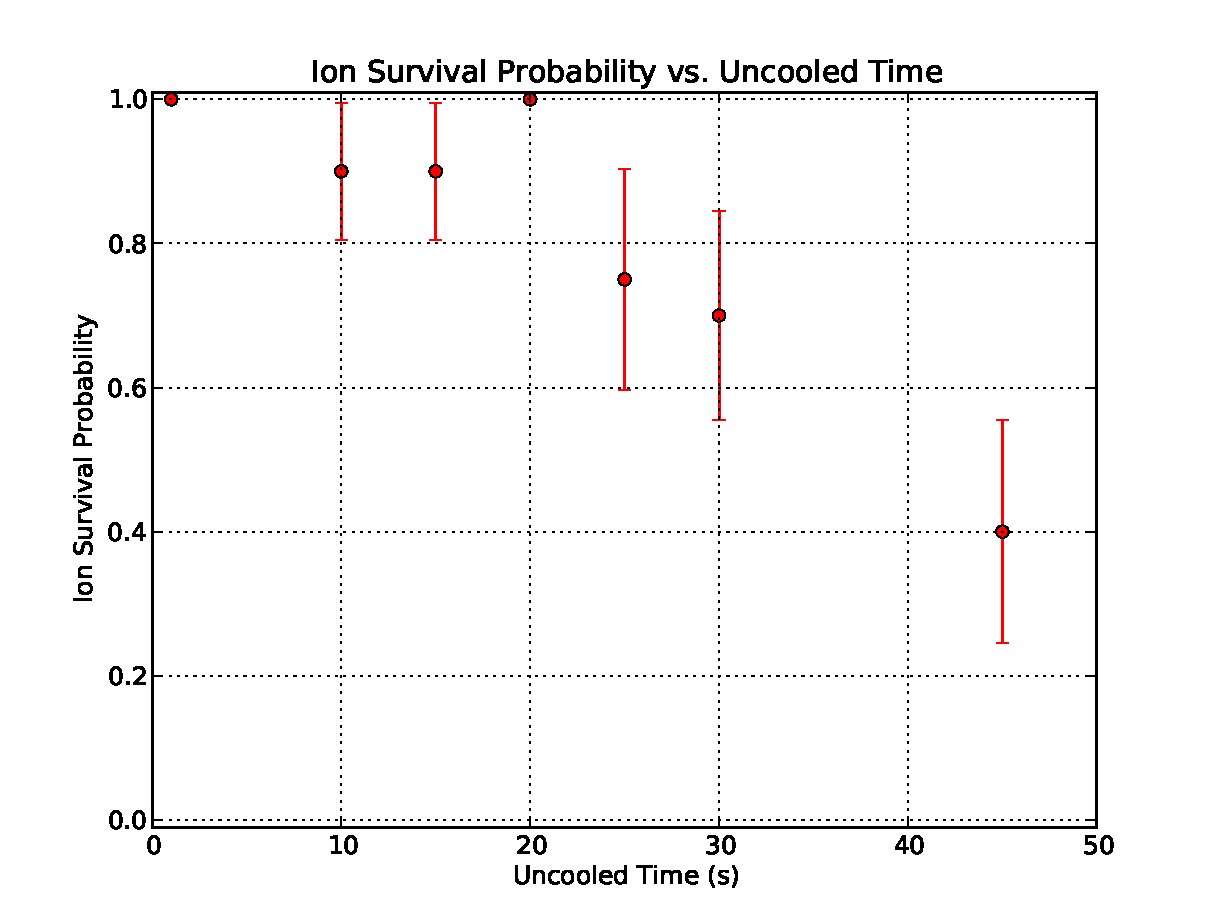
\includegraphics[width=0.7\textwidth]{LifetimeLoadingHole}
	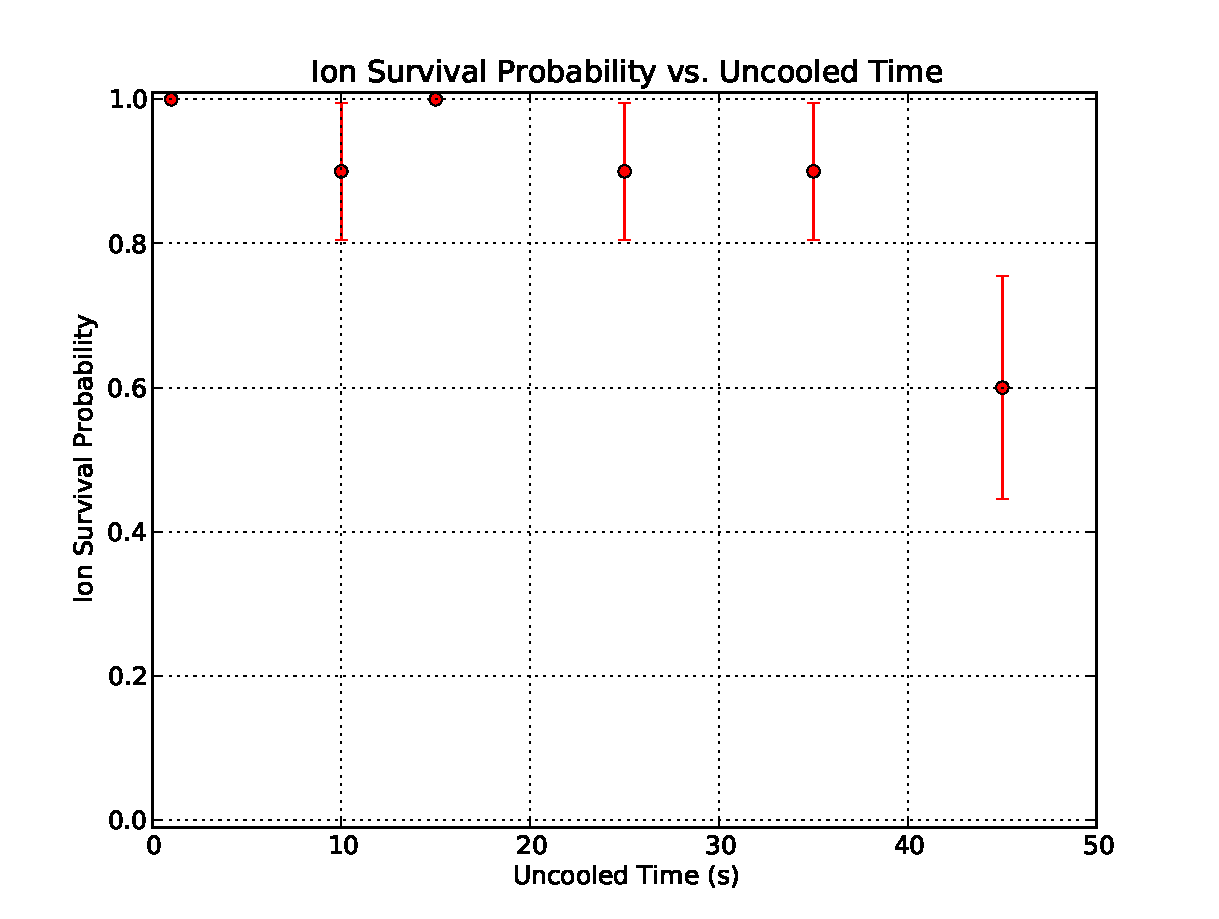
\includegraphics[width=0.7\textwidth]{LifetimeMidarm}
	\caption[Dark lifetime of barium ions in Sandia Y trap]{Dark lifetime of barium ions in a Sandia ``Y'' trap.  The probability that an ion remains trapped and can be recooled after a period of time without Doppler cooling.  This lifetime is significantly shorter in the loading region of the trap (top) than several hundred microns away along the trap (bottom).}
	\label{fig:lifetime}
\end{figure}

Direct heating from electric field noise at the motional secular frequencies has historically been anomalously high.  Heating rates seem to strongly increase as ions are brought closer to surfaces in ion traps, which has made the problem increasingly troublesome as the community moves towards using surface traps where ions are located 40~um to 100~um from the surface of the trap.  The expected scaling for the heating rate as a function of the distance to the nearest surface, $d$, would be $d^{-2}$, but instead there is significant evidence that the dependence is $d^{-4}$.  This problem has often been addressed in the past by using cryogenic instead of room temperature ion trap systems which greatly reduces the electric field noise density \cite{Niedermayr:14, Labaziewicz:08, Chiaverini:14}.  Recent investigations have shown that this surface heating is probably due to electric field noise in contaminants deposited on the surface during the UHV bakeout \cite{Safavi:11,Hite:12}.  These contaminants can be removed by argon ion bombardment after bakeout, which in two separate studies significantly lowered the heating rate in the trap \cite{Hite:12,Daniilidis:14}.

While we are beginning to develop an understanding of the processes behind this heating rate, at the moment it is still one of the most difficult experimental problems in surface traps.  In trapping systems that were not designed to be cleaned by ion bombardment, characterizing and dealing with the trap heating rate is important.

From Figure~\ref{fig:lifetime}, it is clear from our results that there is additional heating near the loading region.  It is beneficial to have regions of the surface trap that do not have loading holes where the heating rates may be lower and quantum operations can be performed more easily.  An additional benefit is that ions can be loaded while quantum operations are being performed without the neutral atom flux perturbing the calculation.  

\section{Secular Frequencies and Stray Fields}
\label{sec:secfreqs}

As discussed in Section~\ref{sec:paul}, the ions' motion can be approximately described as the result of a harmonic potential in each direction.  Measuring the trap frequencies in each direction allows us to characterize the strength of the trapping potential.  A technique to measure these frequencies is to apply a small-amplitude, oscillating electric field and scan its frequency over the possible range for the ions secular frequency.  We can understand the response of the ion to this ``tickle'' voltage by approximating its equation of motion as
\begin{equation}
	\ddot{x} + \omega_x^2 x = \frac{q \vec{E}_t \cdot \hat{x}}{m} \cos( \omega_t x )
\end{equation}
where $\omega_x$ is the radial secular frequency, $q$ is the charge of the ion, $\vec{E}_t$ is the magnitude and polarization of the tickle field, and its angular frequency is $\omega_t$.  This driven harmonic oscillator equation exhibits large amplitude motion when $\omega_t$ is approximately a multiple of $\omega_x$.

Another method for applying the ``tickle'' amplitude is to apply an additional high frequency voltage to the rf electrodes inside the trap.  When this signal's frequency, $\omega_t$, is offset from the applied rf frequency by a multiple of one of the trap frequencies, large amplitude motion can again be observed.  The tickle signal is added to the normal trapping rf using an rf splitter/combiner before the signal is amplified.  Although the rf then passes through a resonator with a Q factor of $\approx$ 200 which acts as a narrow-band filter, enough of the tickle signal remains for the additional motion to be detected.  The advantage of applying the signal this way is that the amplitude of the motional signal the ion sees is minimized when the stray electric field has been compensated, as discussed below. 

The motion of ions in a linear rf trap is given by Equation~\ref{eqn:mathieu-soln} if there is no stray electric field at the trapping location.  Additional micromotion caused by a stray field, $\vec{E}$, adds a term $B_x = q \vec{E} \cdot \hat{x} / m \omega_x^2$ to the solution of the Mathieu equation.  The radial motion of the ions is described by
\begin{equation}
	x(t) = \left( B_x + A_x \cos( \omega_x t + \phi_x ) \right) \left( 1 + \frac{q_x}{2} \cos( \Omega_\mathrm{rf} t ) \right) \mathrm{,}
\end{equation}
where $\Omega_\mathrm{rf}$ is the frequency of the applied rf, $q_x$ is a parameter of the Mathieu equation, and $A_x$ and $\phi_x$ are an amplitude and a phase set by initial conditions.  The larger the motion of the ion at $\Omega_\mathrm{rf}$ due to stray fields, the stronger the Doppler modulated signal from the tickle field it will see at $\omega_t - \Omega_\mathrm{rf}$.  By applying the tickle voltage at $\Omega_\mathrm{rf} + \omega_x$ and minimizing the ions response to it, the micromotion in all three axes can be minimized \cite{Ibaraki:11,Mount:13}.  

The additional motion of the ion caused by either of these tickle voltages can be detected by observing the image of the ion on a CCD camera.  On resonance the amplitude of the ions' motion can increase to $\approx$ 10~$\mu$m distance scales that are easily resolvable.  Since the motion of the ion is much faster than the exposure time of the camera, the ion's image appears to blur out over a larger area while it is being heated and collapse to a small point when cold.  The direction of this blurring can be seen in the CCD images and used to identify the trap axis that is being excited.  Figure~\ref{fig:tickle} shows the ions' response to being driven with an rf tickle near its axial trap frequency.  The additional heating can also be detected by detuning the Doppler cooling laser several linewidths from the transition so that normally the fluorescence is very low.  When the ion is heated it occupies much higher motional states and additional fluorescence can be seen \cite{Mount:13}.

\begin{figure}
	\centering
\begin{tabular*}{0.6\textwidth}{cccc}
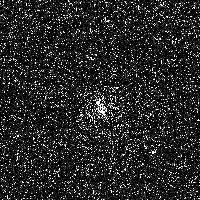
\includegraphics[width=0.1\textwidth]{axial/crop171} &
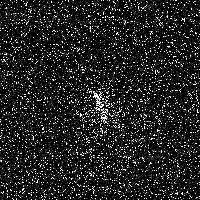
\includegraphics[width=0.1\textwidth]{axial/crop173} &
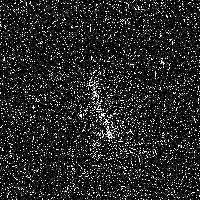
\includegraphics[width=0.1\textwidth]{axial/crop176} &
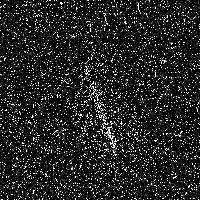
\includegraphics[width=0.1\textwidth]{axial/crop178} \\
{\small 24.171 MHz} & {\small 24.173 MHz} & {\small 24.176 MHz} & {\small 24.178 MHz} \\[0.5in]
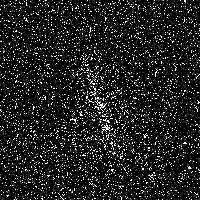
\includegraphics[width=0.1\textwidth]{axial/crop181} &
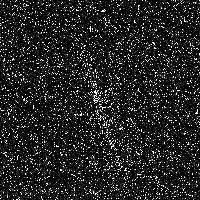
\includegraphics[width=0.1\textwidth]{axial/crop183} &
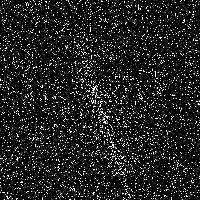
\includegraphics[width=0.1\textwidth]{axial/crop185} &
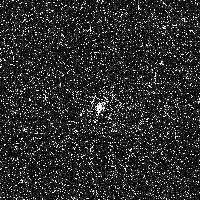
\includegraphics[width=0.1\textwidth]{axial/crop187} \\
{\small 24.181 MHz} & {\small 24.183 MHz} & {\small 24.185 MHz} & {\small 24.187 MHz} \\ 
\end{tabular*}
	\caption[CCD images of a barium ion with resonant rf modulation]{CCD images of a single \ba ion at different applied rf tickle frequency indicated underneath each image. The trap rf frequency, $\Omega_\mathrm{rf}$, was 24.93~MHz.  The amplitude of the ions motion increases dramatically when the tickle frequency is offset from the carrier frequency by a multiple of the trap frequencies.  The excitation shown is the trap axial mode which in these images is oriented along an axis approximately 30 degrees counter-clockwise  from vertical.}
	\label{fig:tickle}
\end{figure}

Using this measurement technique we have measured the secular frequencies of our trap with the voltages we are currently applying.  The axial angular frequency is $\approx$ 2$\pi \times$ 0.75~MHz using dc voltages of order $\pm$ 5~V, and the radial frequencies are $\approx$ 2$\pi \times$ 1.50~MHz and 2$\pi \times$ 2.05~MHz with approximately 100~Vpp of 20~MHz rf.  


